\documentclass[titlepage]{report}
\title{Amazon Web Services:\\ EC2\hyp{}virtual\hyp{}server und EC2\hyp{}container \\
\small Eine Seminar\hyp{}Arbeit bei Prof. Dr. -Ing. Dr. rer. nat. habil. \\
Harald Richter}
\usepackage[ngerman]{babel}
\usepackage[backend=biber,style=numeric]{biblatex}
\addbibresource{literature.bib}
\usepackage{caption}
\usepackage{subcaption}
\usepackage{graphicx}
\usepackage[utf8]{inputenc}
\usepackage[T1]{fontenc}
\usepackage{url}
\usepackage{hyphenat}
\author{Christian, Rebischke}
\begin{document}
\maketitle
\tableofcontents
\chapter*{Einleitung}
\addcontentsline{toc}{chapter}{Einleitung}
Im Zeitalter immer fortschreitender Digitalisierung wächst die Nachfrage
nach günstigem Speicherplatz und Rechenpower zunehmends. Der Trend geht
deshalb immer mehr zum Cloud Computing.  ``Zwei von drei Unternehmen (65
Prozent) haben in Deutschland im Jahr 2016 Cloud Computing
eingesetzt.''\footcite{SWG17} Cloud Computing ist die Möglichkeit
Speicher und Rechenpower in Form von Cloud\hyp{}Storage, virtuellen Servern,
der neuen Container\hyp{}Technologie oder ganzen Rechenzentren on\hyp{}demand
virtuell abzurufen, zu verwalten und für die eigene Firma möglichst
schlagkräftig zu verwenden. Die Vorteile dieses neuen Marktsegments sind
offensichtlich. So lassen sich Anwendungen jederzeit und an jedem Ort
der Welt deployen und einfach skalieren, so fern es der Cloud\hyp{}Anbieter
möglich macht durch Rechenzentren, verteilt über den gesamten Globus.
Dies ermöglicht ein rasantes Wachstum für neue Startups, kleine und
mittelständische Unternehmen sowie große Konglomerate wie Amazon oder
Microsoft wie es die Welt noch nie zuvor gesehen hat. Startups oder
bereits etablierte Firmen sparen sich auf diesem Wege den Overhead
eigene Hardware zu kaufen und zu verwalten.  Eigene Hardware hat den
Nachteil der Skalierbarkeit. Als Startup mit beispielsweise gerade mal
ein Dutzend Mitarbeitern ist es unmöglich weltweit zu skalieren auf
Basis von Hardware. Der Einkauf und die anschließende Verwaltung von
Servern, Routern, Storages oder Switches ist nicht nur kostenintensiv,
sondern vorallem auch zeit\hyp{} und Mitarbeiterintensiv.\footcite[S.
1]{RZ17} Besonders wenn man weltweit expandieren möchte ist es enorm
schwerig für Newcomer genug Infrastruktur aufzubauen um alle Kunden
zufriedenstellend zu versorgen.  So kann zum Beispiel eine Verbindung
zwischen dem Rechenzentrum einer Firma in München und einem Kunden in
Berlin zufriedenstellend sein. Ein Kunde in Asien jedoch, beispielsweise
China, hätte mit starker Latenz zu kämpfen. Ein weiteres Beispiel
Redundanz: Mit steigender Kundschaft steigt auch die Wahrscheinlichkeit
das Server ausfallen. Das kann viele Gründe haben. Hardware\hyp{}Ausfall,
Fehler in der Administration oder Überlastung wegen eines zu hohen Loads
auf dem Server sind nur wenige Gründe. Die Antwort darauf ist
horizontales Skalieren. Anstatt vertikal zu skalieren und mehr
Rechenpower und Speicher in nur eine Server\hyp{}Einheit zu stecken ist es
ratsamer die Last und damit auch das Ausfall\hyp{}Risiko auf mehrere Servern
zu verteilen. Im Idealfall sind diese Server sogar noch physisch von
einander getrennt um Ausfälle durch Naturkatastrophen oder politischen
Auseinandersetzungen zu vermeiden.  Alle diese Ansätze vereint Amazon
Web Services (AWS). Im weiteren Verlauf dieser Arbeit wird der Dienst
Amazon EC2 genauer vorgestellt und dessen Kernkonzepte Virtual\hyp{}Server
und Container genauer beleuchtet. Außerdem werden etwaige Vorteile und
Nachteile sowie Unterschiede zwischen beiden Konzepten hervorgehoben.
\begin{figure}[h]
    \centering
    \includegraphics[width=1.0\textwidth]{figures/scalability.pdf}
    \caption{Verdeutlichung Horizontaler Skalierung}\label{fig:1}
\end{figure}
\chapter*{Amazon EC2}
\addcontentsline{toc}{chapter}{Amazon EC2}
\section*{Einführung in Amazon EC2}
\addcontentsline{toc}{section}{Einführung in Amazon EC2}
Amazon EC2, ausgeschrieben Amazon Elastic Compute Cloud, ist im Jahr
2006 als Bestandteil von Amazon Web Services (AWS)
entstanden.\footcite{aws} Amazon Web Services gehört dem gleichnamigen
Tochterunternehmen des Online\hyp{}Versandhändlers Amazon.com.\footcite{Fou}
Das Tochterunternehmen deckt verschiedene Sparten des Cloud\hyp{}Computing
ab. Darunter fallen diverse Bereiche wie Rechenpower in Form von
virtuellen Servern und Containern, Speicher in Form des Amazon Web
Service S3 (Simple Storage Service) oder des Datenbank\hyp{}Services Amazon
RDS (Relational Database Service) oder Netzwerk in Form von CloudFront,
einem Content Delivery Network von Amazon Web Services. Weitere Dienste
sind zum Beispiel IAM (Identity and Access Managament), Lightsail oder Beanstalk.
Damit sind noch lange nicht alle Services genannt. In dieser Arbeit soll
es aber explizit um Amazon EC2 (Elastic Compute Cloud) gehen. Einige der
Hauptmerkmale von Amazon Elastic Compute Cloud sind:
\begin{itemize}
    \item Hohe Skalierbarkeit
    \item Webservice mit API
    \item Instanzen sind On\hyp{}Demand verfügbar innerhalb von Minuten anstatt
      Stunden oder Tagen
    \item Service Level Agreement garantiert 99,95\% uptime\footcite{ec2}
    \item Rechenzentren in verschiedenen Regionen der Welt
    \item Integration in andere Amazon Web Services: Zum Beispiel S3
    \item Kostengünstig: Es wird nur für genutzte Rechenkapazität bezahlt
\end{itemize}
Wenn man von Amazon EC2 spricht, spricht man fast immer von virtuellen
Maschinen in der Amazon Web Services Cloud. Als Grundlage für diese
virtuellen Maschinen oder auch Instanzen (englisch Instance) dienen
Amazon Machine Images (AMI).\footcite{ec2details} Amazon Machine Images
können verschiedene Betriebssysteme beinhalten. Angefangen bei Microsoft
Windows über diverse Linux Derivate wie Red Hat Linux (RHEL), Debian
oder CentOS. Anhand von diesen AMIs lassen sich dann wiederum Instanzen
starten. Kosten werden nur verursacht während eine Instanz gestartet
ist. (Bei einigen Amazon Machine Images können Lizenzkosten anfallen,
zum Beispiel Windows). Desweiteren lassen sich Amazon Machine Images
beliebig konfigurieren. Diese Konfiguration umfasst aber nur
Einstellungen auf Betriebssystemebene. Um Parameter wie CPU, RAM,
Speicher oder Netzwerk einzustellen bietet Amazon Web Services eine
Palette von Instanztypen (englisch Instance\hyp{}Types) an.  Diese
Instanztypen decken ein breites Spektrum von unterschiedlichen
Konfigurationen ab. Angefangen beim kleinsten Instanztyp dem T2.nano mit
einem virtuellen CPU\hyp{}Kern und 0.5GiB Arbeitsspeicher bis hin zum
größten Instanztyp wie dem m4.16xlarge mit 64 virtuellen
CPU\hyp{}Kernen, 256GiB Arbeitsspeicher und einer dedizierten
EBS\hyp{}Bandbreite von 10.000 Mbit/s.  \footcite{instance} EBS steht
für Elastic Block Store und ist eine dedizierte Speichereinheit in der
Amazon Web Services Cloud. Elastic Block Store kann auf jede beliebige
Größe angepasst werden und ist unabhängig von der Elastic Compute Cloud.
So überlebt Elastic Block Store beispielsweise einen Reboot der
virtuellen Maschine und kann auch an andere Instanzen
angedockt/gemounted werden. Durch diese Eigenschaft ist es möglich ohne
Probleme innerhalb von Minuten von einer Instanz auf eine andere
umzuziehen.
\begin{table}[h]
    \centering
    \caption{Beispiel für die Varianz der Instanzen anhand vom Typ T2\footcite{instance}}
    \label{tab:1}
\begin{tabular}{|c|c|c|c|c|}
\hline
Modell     & vCPU & CPU\hyp{}Guthaben/Stunde & Arbeitsspeicher (GiB) & Speicherung \\ \hline
t2.nano    & 1    & 3                   & 0.5                   & Nur EBS     \\
t2.micro   & 1    & 6                   & 1                     & Nur EBS     \\
t2.small   & 1    & 12                  & 2                     & Nur EBS     \\
t2.medium  & 2    & 24                  & 4                     & Nur EBS     \\
t2.large   & 2    & 36                  & 8                     & Nur EBS     \\
t2.xlarge  & 4    & 54                  & 16                    & Nur EBS     \\
t2.2xlarge & 8    & 81                  & 32                    & Nur EBS     \\ \hline
\end{tabular}
\end{table}
\newpage
Die Namensgebung der verschiedenen Instanzen folgt einem festen Muster.
Eine Instanzfamilie bezeichnet die verschiedenen
Instanz\hyp{}Optimierungen in Bezug auf GPU,CPU,Netzwerk oder Speicher.
Die Instanzgenerationen unterscheiden sich zum Beispiel durch den
Einsatz von Virtualisierungstechniken oder anderen Features. Die
Instanzgröße wiederum bezeichnet die Ausstattung der Instanz im Bezug
auf numerische Werte wie die Anzahl der virtuellen CPU\hyp{}Kerne,
Arbeitsspeicher, Netzwerk etc.
\begin{figure}[h]
    \centering
    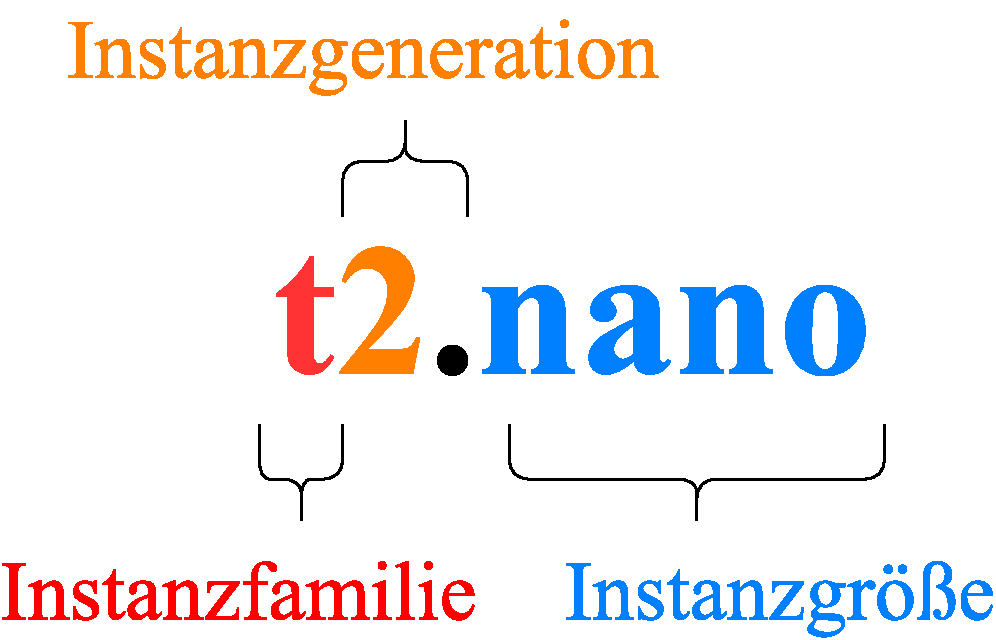
\includegraphics[width=0.5\textwidth]{figures/instance.pdf}
    \caption{Erläuterung der Amazon Instance Namensgebung}\label{fig:2}
\end{figure}
\begin{figure}[h]
    \centering
    \includegraphics[width=1.0\textwidth]{figures/EC2-Landscape.pdf}
    \caption{Übersicht über die EC2\hyp{}Instanz\hyp{}Landschaft}\label{fig:3}
\end{figure}
\newpage
\section*{Regionen}
\addcontentsline{toc}{section}{Regionen}
Um eine weitgefächerte Verfügbarkeit und Skalierbarkeit zu gewährleisten
hat Amazon Web Services Rechenzentren in einem Dutzend Ländern. Dadurch
ist es möglich die Latenz und Fehlerquote von Webseiten und internetbasierten
Anwendungen so klein wie möglich zu halten. Dies hat nicht nur eine
höhere Kundenzufriedenheit zur Folge sondern hat auch technische
Vorteile (beispielsweise für Video\hyp{}Anwendungen). Zur Zeit unterhält
Amazon Web Services Rechenzentren in den folgenden Ländern:
\begin{itemize}
    \item USA
    \item Deutschland
    \item Volksrepublik China
    \item Irland
    \item Großbritannien
    \item Indien
    \item Südkorea
    \item Australien
    \item Japan
    \item Singapur
    \item Kanada
    \item Brasilien
\end{itemize}
Diese Länder sind eingeteilt in folgende geographische Regionen:
\begin{itemize}
    \item Nordamerika
    \item Europa/Naher Osten/Afrika
    \item Asien/Pazifik
    \item Südamerika
\end{itemize}
Damit sind bis auf den Kontinent Afrika, alle besiedelten Kontinente
abgedeckt. Diese geographischen Regionen sind dann nochmal in Regionen
unterteilt. Für Nordamerika wären das beispielsweise\footcite{region}:
\begin{itemize}
    \item USA Ost (Nord\hyp{}Virginia)
    \item USA Ost (Ohio)
    \item USA West (Oregon)
    \item USA West (Nordkalifornien)
    \item Kanada
    \item AWS GovCloud
\end{itemize}
AWS GovCloud ist eine Sonder\hyp{}Region und isoliert von allen anderen
Regionen. Der Grund dafür ist, dass AWS GovCloud Applikationen und
Informationen der US\hyp{}Regierung hosted.\footcite{govcloud} Zusätzlich zu
diesen Regionen gibt es noch High\hyp{}Availability\hyp{}Zones
(Hoch\hyp{}Verfügbarkeits\hyp{}Zonen). Eine Region kann mehrere dieser
High\hyp{}Availability\hyp{}Zonen haben. Im Endeffekt handelt es sich bei
diesen Zonen um physische Rechenzentren in verschiedenen Städten innerhalb
einer Region. Die Region USA Ost (Nord Virginia) hat beispielsweise 5
High\hyp{}Availability\hyp{}Zonen. Durch diese
High\hyp{}Availability\hyp{}Zonen kann man Applikationen mehrfach in einer
Region deployen, dadurch erhält man automatische, unterbrechungsfreie Failover
die zu einer hohen Redundanz führen.\footcite{region} Realisiert wird dies
durch private Glasfasernetzwerke zwischen den einzelnen
High\hyp{}Availability\hyp{}Zonen. Dies lässt sich dann weiter hochskalieren
über ganze Regionen. Außerdem gibt es noch
AWS\hyp{}Edge\hyp{}Network\hyp{}Standorte. Dies sind meistens Standorte für
Content\hyp{}Delivery\hyp{}Netzwerke, kleinere Rechenzentren oder
Peering\hyp{}Endpunkte.
\section*{Virtualisierung}
\addcontentsline{toc}{section}{Virtualisierung}
Einer der Schlüsselfaktoren für die gute Skalierbarkeit von Amazon EC2
ist die Virtualisierung. Durch den Einsatz von Virtualisierung ist es
möglich mehrere virtuelle Hosts auf einer Hardware laufen zu lassen.
Das Prinzip dahinter ist relativ simpel. Auf dem OS der Hardware läuft
ein Hypervisor oder auch Virtual Machine Monitor (VMM). Über diesen
Hypervisor können dann mehrere Instanzen von virtuellen Servern auf der
selben Hardware gestartet werden. Der Hypervisor gaukelt den einzelnen
Maschinen also vor, sie wären nur auf einem System.
\begin{figure}[h]
    \centering
    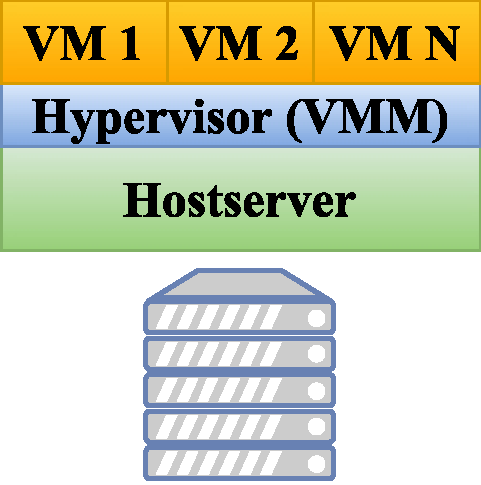
\includegraphics[width=0.5\textwidth]{figures/hypervisor.pdf}
    \caption{Visualisierung der Hypervisor\hyp{}Technologie}\label{fig:4}
\end{figure}
\\
Amazon Machine Images unterstützen zwei verschiedene Arten von
Virtualisierung:
\begin{itemize}
    \item paravirtual (PV)
    \item hardware virtual machine (HVM)
\end{itemize}
``Der Hauptunterschied zwischen PV und HVM basierten Amazon Machine
Images besteht im verwendeten Bootloader und der Verfügbarkeit von
speziellen Hardware\hyp{}Erweiterungen (CPU, Netzwerk, Speicher) für bessere
Performance.''\footcite{virtualization} Bei PV basierten Amazon Machine
Images wird also keine Hardware\hyp{}Emulation benutzt. Dies bedeutet im
Umkehrschluss, dass das jeweilige Betriebssystem in der virtuellen Maschine nur
software\hyp{}seitig emuliert wird. Dadurch hat die VM dann auch keinen
direkten Zugang zur Hardware und wird dazu gezwungen den Umweg über den
Hypervisor zu nehmen, dies kostet Ressourcen und mindert die
Performance. Vorteil an PV basierten Hosts ist allerdings, dass die
Hardware keinen Support für Virtualisierung benötigt. (Dies ist meistens
bei älterer oder sehr billiger Hardware der Fall). Hinzukommend nutzen
PV basierte AMIs einen speziellen Bootloader (eine gepatchte Version des
bekannten Linux Bootloaders GRUB), welcher den Boot\hyp{}Zyklus in
Gang setzt und danach den richtigen Kernel
lädt.\footcite{virtualization} Bei HVM basierten Amazon Machine Images
hingegen virtualisiert die Hardware die Gast\hyp{}Systeme (dies geschieht
beispielsweise durch die Intel Virtualization Technology (Intel VT\hyp{}x)).
Dies hat nicht nur eine bessere Performance der virtualisierten
Instanzen zur Folge sondern ermöglicht auch den direkten Zugriff auf
einzelne Hardware\hyp{}Komponenten wie beispielsweise GPU oder Netzwerk.
\begin{figure}[h]
    \centering
    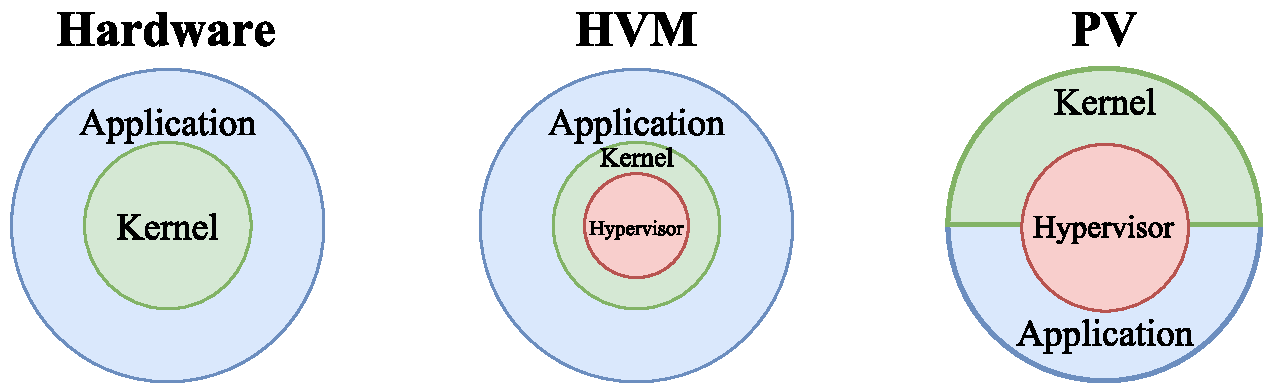
\includegraphics[width=1.0\textwidth]{figures/hvm_pv.pdf}
    \caption{HVM und PV im Vergleich}\label{fig:5}
\end{figure}
\section*{EC2 container}
\addcontentsline{toc}{section}{EC2 container}
Als Ergänzung zu den hardware\hyp{} und paravirtualisierten Instanzen
bietet Amazon Web Services unter dem Produktnamen ``EC2 container'' auch
Container an. Container sind keine virtuellen Maschinen. Stattdessen
basieren die bei Amazon Web Services eingesetzten Container auf der
Docker\hyp{}Technologie. Docker ist eine Opensource\hyp{}Software welche
anhand von Betriebssystem\hyp{}Kernel\hyp{}Features einzelne Anwendungen
und dessen benötigte Bibliotheken sowie ganze Betriebssysteme isolieren
kann. Dadurch ist es möglich ohne Virtualisierung auf einem Host mehrere
Container mit mehreren Einsatzwecken auszuführen. Dies kann zum Beispiel
eine einzelne Webanwendung sein oder ein ganzes Linux-Betriebssystem.
Die Rolle des Hypervisors übernimmt stattdessen der Docker\hyp{}Daemon oder
die Docker\hyp{}Engine. Als Host\hyp{}System kann ein Microsoft Windows
oder ein Linux eingesetzt werden. Auf Linux nutzt Docker folgende
Kernel\hyp{}Features zum isolieren des Docker\hyp{}Containers vom
restlichen Betriebssystem:
\begin{itemize}
    \item Namespaces
    \item Control groups
    \item Union file systems
\end{itemize}
Bei Namespaces handelt es sich um eine Prozess\hyp{}Virtualisierung.
Statt einem festen Hypervisor wie beispielsweise KVM oder Xen wird dafür
der system call ``setns()'' des Linux\hyp{}Kernels benutzt. Der
``setns()''\hyp{}syscall existiert im Linux\hyp{}Kernel seit Version
3.0.\footcite{setns} Die Prozess\hyp{}Virtualisierung ist nichts anderes als
eine Prozess\hyp{}Isolation. Ein Prozess hat also nur eine eingeschränkte
Sichtweite und kann nur innerhalb seines zugewiesenen Namespaces
agieren. Docker benutzt die folgenden 5 Namespaces:\footcite{docker}
\begin{itemize}
    \item The ipc namespace
    \item The net namespace
    \item The pid namespace
    \item The mnt namespace
    \item The uts namespace
\end{itemize}
Der \textbf{ipc} Namespace regelt den Zugriff auf Ressourcen für
Interprozesskommunikation. Da der Linux\hyp{}Kernel immer noch keine
Interprozesskommunikation auf Kernel\hyp{}Ebene besitzt werden die
üblichen Ressourcen dafür benutzt. Also Sockets, Shared Memory und
Pipes.\footcite{ipc} Der \textbf{net} Namespace managed den Zugriff auf
Netzwerk\hyp{}Ressourcen wie beispielsweise Ethernet\hyp{} oder
WLAN\hyp{}Interfaces. Der \textbf{pid} Namespace ist wiederum für die
Prozess\hyp{}Isolation zuständig. Dazu wird praktisch innerhalb eines
Prozesses ein eigener Prozess\hyp{}Namespace angelegt in dem dann nach
belieben weitere isolierte Prozesse gespawned werden können. Beim
\textbf{mnt} Namespace werden die Mount\hyp{}Points im Filesystem
isoliert. Dadurch stellt der Docker\hyp{}Daemon sicher, dass die
einzelnen isolierten Container auch wirklich nur Zugriff auf die Teile
des Filesystems haben auf die sie auch Zugriff haben sollen. Der letzte
für Docker wichtige Namespace, der \textbf{uts} Namespace isoliert den
Kernel und sorgt für die richtige Zeit in den Containern. Eine korrekte
Unix\hyp{}Zeit ist enorm wichtig für ordentliche Kryptographie und
verteilte Anwendungen. Ein weiteres wichtiges Kernel\hyp{}Feature für
Container unter Linux sind Control Groups. Control Groups oder auch
\textbf{cgroups} isolieren Ressourcen für eine Gruppe von
Prozessen.\footcite{cgroups} \textbf{cgroups} können dafür auf
Namespaces zur Isolation zurück greifen. Außerdem sind Union file
systems essentiell für Docker\hyp{}basierte Systeme. Union file systems
ist ein Sammelbegriff für Filesysteme die das Filesystem in Schichten
unterteilen. Darunter fallen zum Beispiel btrfs, AUFS, vfs oder
DeviceMapper.\footcite{docker}
Dadurch, dass bei Containern keine Virtualisierung stattfindet sondern
nur eine Prozess\hyp{}Isolierung wird beim Einsatz von Containern viel
weniger Ressourcen benutzt als bei gängigen Virtualisierungstechniken.
Mit diesem Ansatz lassen sich ganze Cluster bauen aus mehreren
Containern und kann so einzelne Applikationen oder Bausteine einer
größeren Anwendung gezielt kapseln und Einzelteile austauschen oder
andersweitig modifizieren. (Zum Beispiel durch die Zuweisung von mehr
Ressourcen). Außerdem ist im Entwicklungsprozess einer Anwendung es
möglich, wenn Container verwendet werden, eine Anwendung einfacher in
eine Cloud\hyp{}Umgebung einzupflegen. Es muss nur noch der Container an
der richtigen Stelle platziert werden. Dieser Container bringt dann im
Idealfall alle Abhängigkeiten für die genannte Anwendung mit und es muss
nicht zu erst aufwendig eine virtuelle Maschine provisioniert und an die
Anwendung angepasst werden. Zusätzlich lassen sich Container von
Entwicklern einfacher importieren. So erspart man sich das Aufsetzen
einer Entwicklungsumgebung mit allen Eigenheiten der zu entwickelnden
Applikation. Amazon EC2 Container verfeinert diese Vorzüge von
Containern sogar noch. Einige der Vorzüge von EC2 Container
sind:\footcite{container}
\begin{itemize}
    \item Einfaches Cluster Management
    \item Hohe Performance
    \item Flexibles Scheduling
    \item Erweiterbarkeit und Portierbarkeit
    \item Ressourceneffizienz
    \item Integration in andere AWS\hyp{}Dienste
    \item Sicherheit durch Integration in Amazon Virtual\hyp{}Private\hyp{}Cloud
\end{itemize}
\section*{Sicherheit}
\addcontentsline{toc}{section}{Sicherheit}
Eine wichtige Eigenschaft von Cloud\hyp{}Umgebungen ist die Sicherheit.
Keine Firma würde ihre Daten oder ihre Infrastruktur in eine Cloud
legen, wenn die Firma wüsste, dass die Cloud anfällig gegen Hacker ist.
Amazon Web Services versucht es Hackern so schwierig wie möglich zu
machen. So bietet Amazon Web Services reichlich Informationsmaterial zu
dem Thema, bietet die Möglichkeit von
Penetrationstests\footcite{penetration}, eine Kontaktadresse um
Schwachstellen zu melden und diverse Sicherheits\hyp{}Features. Alles
Dinge die heutzutage nicht ganz selbstverständlich sind aber
selbstverständlich sein sollten.  Amazon Machine Images werden
beispielsweise wenn diese via SSH (SecureShell) gewartet werden stehts
mit SSH\hyp{}Keys statt Plaintext\hyp{}Passwörtern abgesichert.
SSH\hyp{}Keys sind Plaintext\hyp{}Passwörtern in vieler Hinsicht
überlegen. Erstens neigt man nicht dazu einfache Passwörter zu gestalten
und zweitens hat man bei SSH\hyp{}Keys mehr Komponenten. Ein
SSH\hyp{}Key besteht immer aus zwei Teilen. Einem privaten und einem
öffentlichen Schlüssel. Der private Schlüssel ist meistens noch mit
einem Kennwort abgesichert als zusätzliche Hürde für den Angreifer. Der
öffentliche Schlüssel wird auf einem virtuellen Server oder Container
abgelegt, der private Schlüssel ist im Besitz des Administrators. Amazon
Web Services bietet diese Möglichkeit solche SSH\hyp{}Keys im Browser zu
generieren oder man verwendet eigene Keys. Letzteres stellt sicher, dass
selbst Amazon nicht im Besitz des privaten Schlüssels ist, selbst wenn
Amazon dazu in der Lage wäre den im Browser generierten privaten
Schlüssel abzufangen.  Desweiteren bietet Amazon Web Services die
Möglichkeit \textbf{s3}\hyp{}Instanzen zu verschlüsseln. Dies kann
server\hyp{}seitig von Amazon aus passieren oder client\hyp{}seitig vom
jeweiligen Benutzer des Dienstes.\footcite{encryption} Letzteres ist mit
einem erhöhten Aufwand verbunden. Desweiteren unterstützt Amazon Web
Services für viele seiner Dienste
Multi\hyp{}Faktor\hyp{}Authentifizierung (MFA). Zur Wahl stehen
SMS\hyp{}basierte Lösungen oder Security\hyp{}Tokens. Für
Security\hyp{}Tokens benötigt man ein MFA\hyp{}Gerät, dies kann zum
Beispiel ein Smartphone sein oder auch virtualisiert
werden.\footcite{mfa}Zwei weitere Schlüssel\hyp{}Konzepte für Sicherheit
in der AWS Cloud sind: Amazon Identity and Access Management (IAM) und
Amazon Security Groups. Bei Amazon Identity and Access Management
handelt es sich um eine zentrale Verwaltung um den Zugang auf einzelne
Instanzen oder Amazon Produkte via Benutzer\hyp{} oder
Gruppenrichtlinien zu verwalten.\footcite{iam} Die Verwaltung läuft
dabei via Weboberfläche oder in der Shell mit dem AWS\hyp{}Client.
Für Netzwerksicherheit setzt Amazon Web Services auf Security Groups.
Diese Security Groups haben gegenüber einer traditionellen Firewall
einige Vorteile. Normalerweise legt man nämlich eine Firewall über ein
komplettes Subnetz und riegelt damit das betreffende Subnetz von außen
ab. Durch diese Maßnahme steigen jedoch die Anzahl der
Firewall\hyp{}Regeln und dessen Komplexität. Dies macht nicht nur
Debugging kompliziert sondern auch das erstellen von neuen Regeln, da
Regeln immer global gelten für das komplette Subnetz. Amazon Web
Services Lösung sind Security Groups. Anhand von Security Groups kann
man Firewall\hyp{}Regeln einer Gruppe von Instanzen mit den gleichen
Aufgaben zuweisen. Diese vergebenen Regeln betrffen dann jeweils nur
diese Instanz und gelten nicht global für alle Instanzen. Außerdem gilt
bei Amazon Security Groups, dass ausgehender Traffic immer erlaubt ist
und einkommender Traffic präventiv geblockt wird. Dieser Mechanismus
gewährleistet maximale Sicherheit mit möglichst geringer Komplexität da
weniger Regeln gebraucht werden. Die unten abgebildeten Grafiken
verdeutlichen dieses Prinzip nochmal.
\begin{figure}[h]
      \centering
      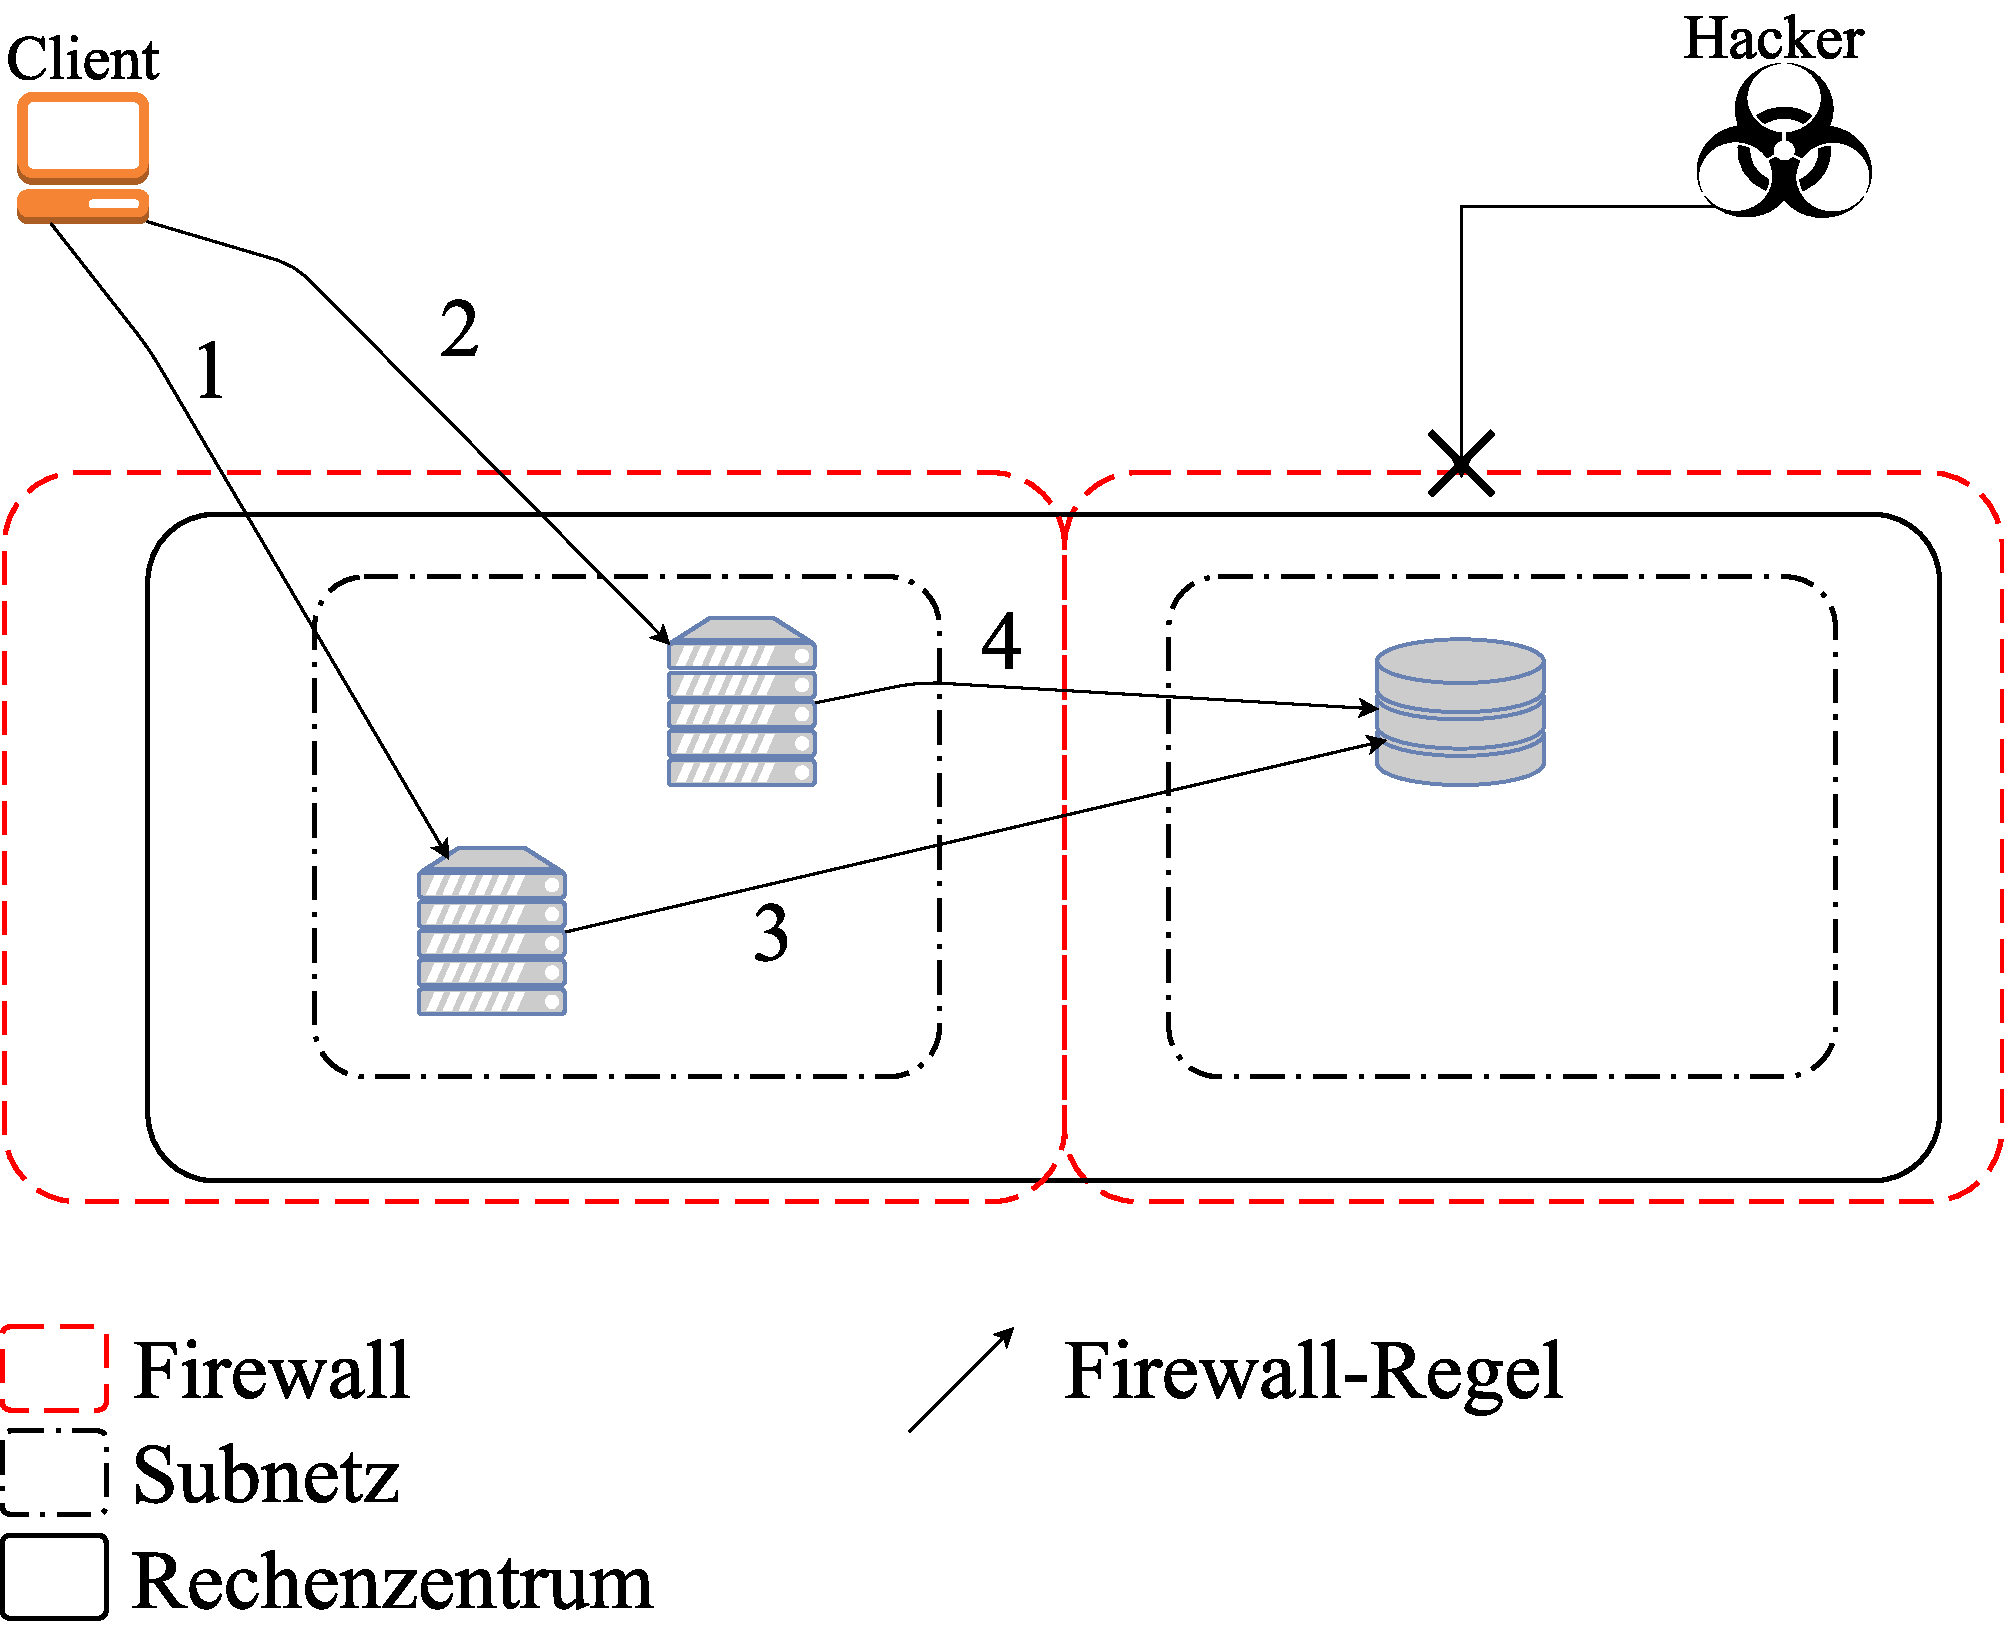
\includegraphics[width=0.8\textwidth]{figures/traditional_firewall.pdf}
      \caption{Traditionelle Firewall}\label{fig:6}
\end{figure}
\begin{figure}[h]
      \centering
      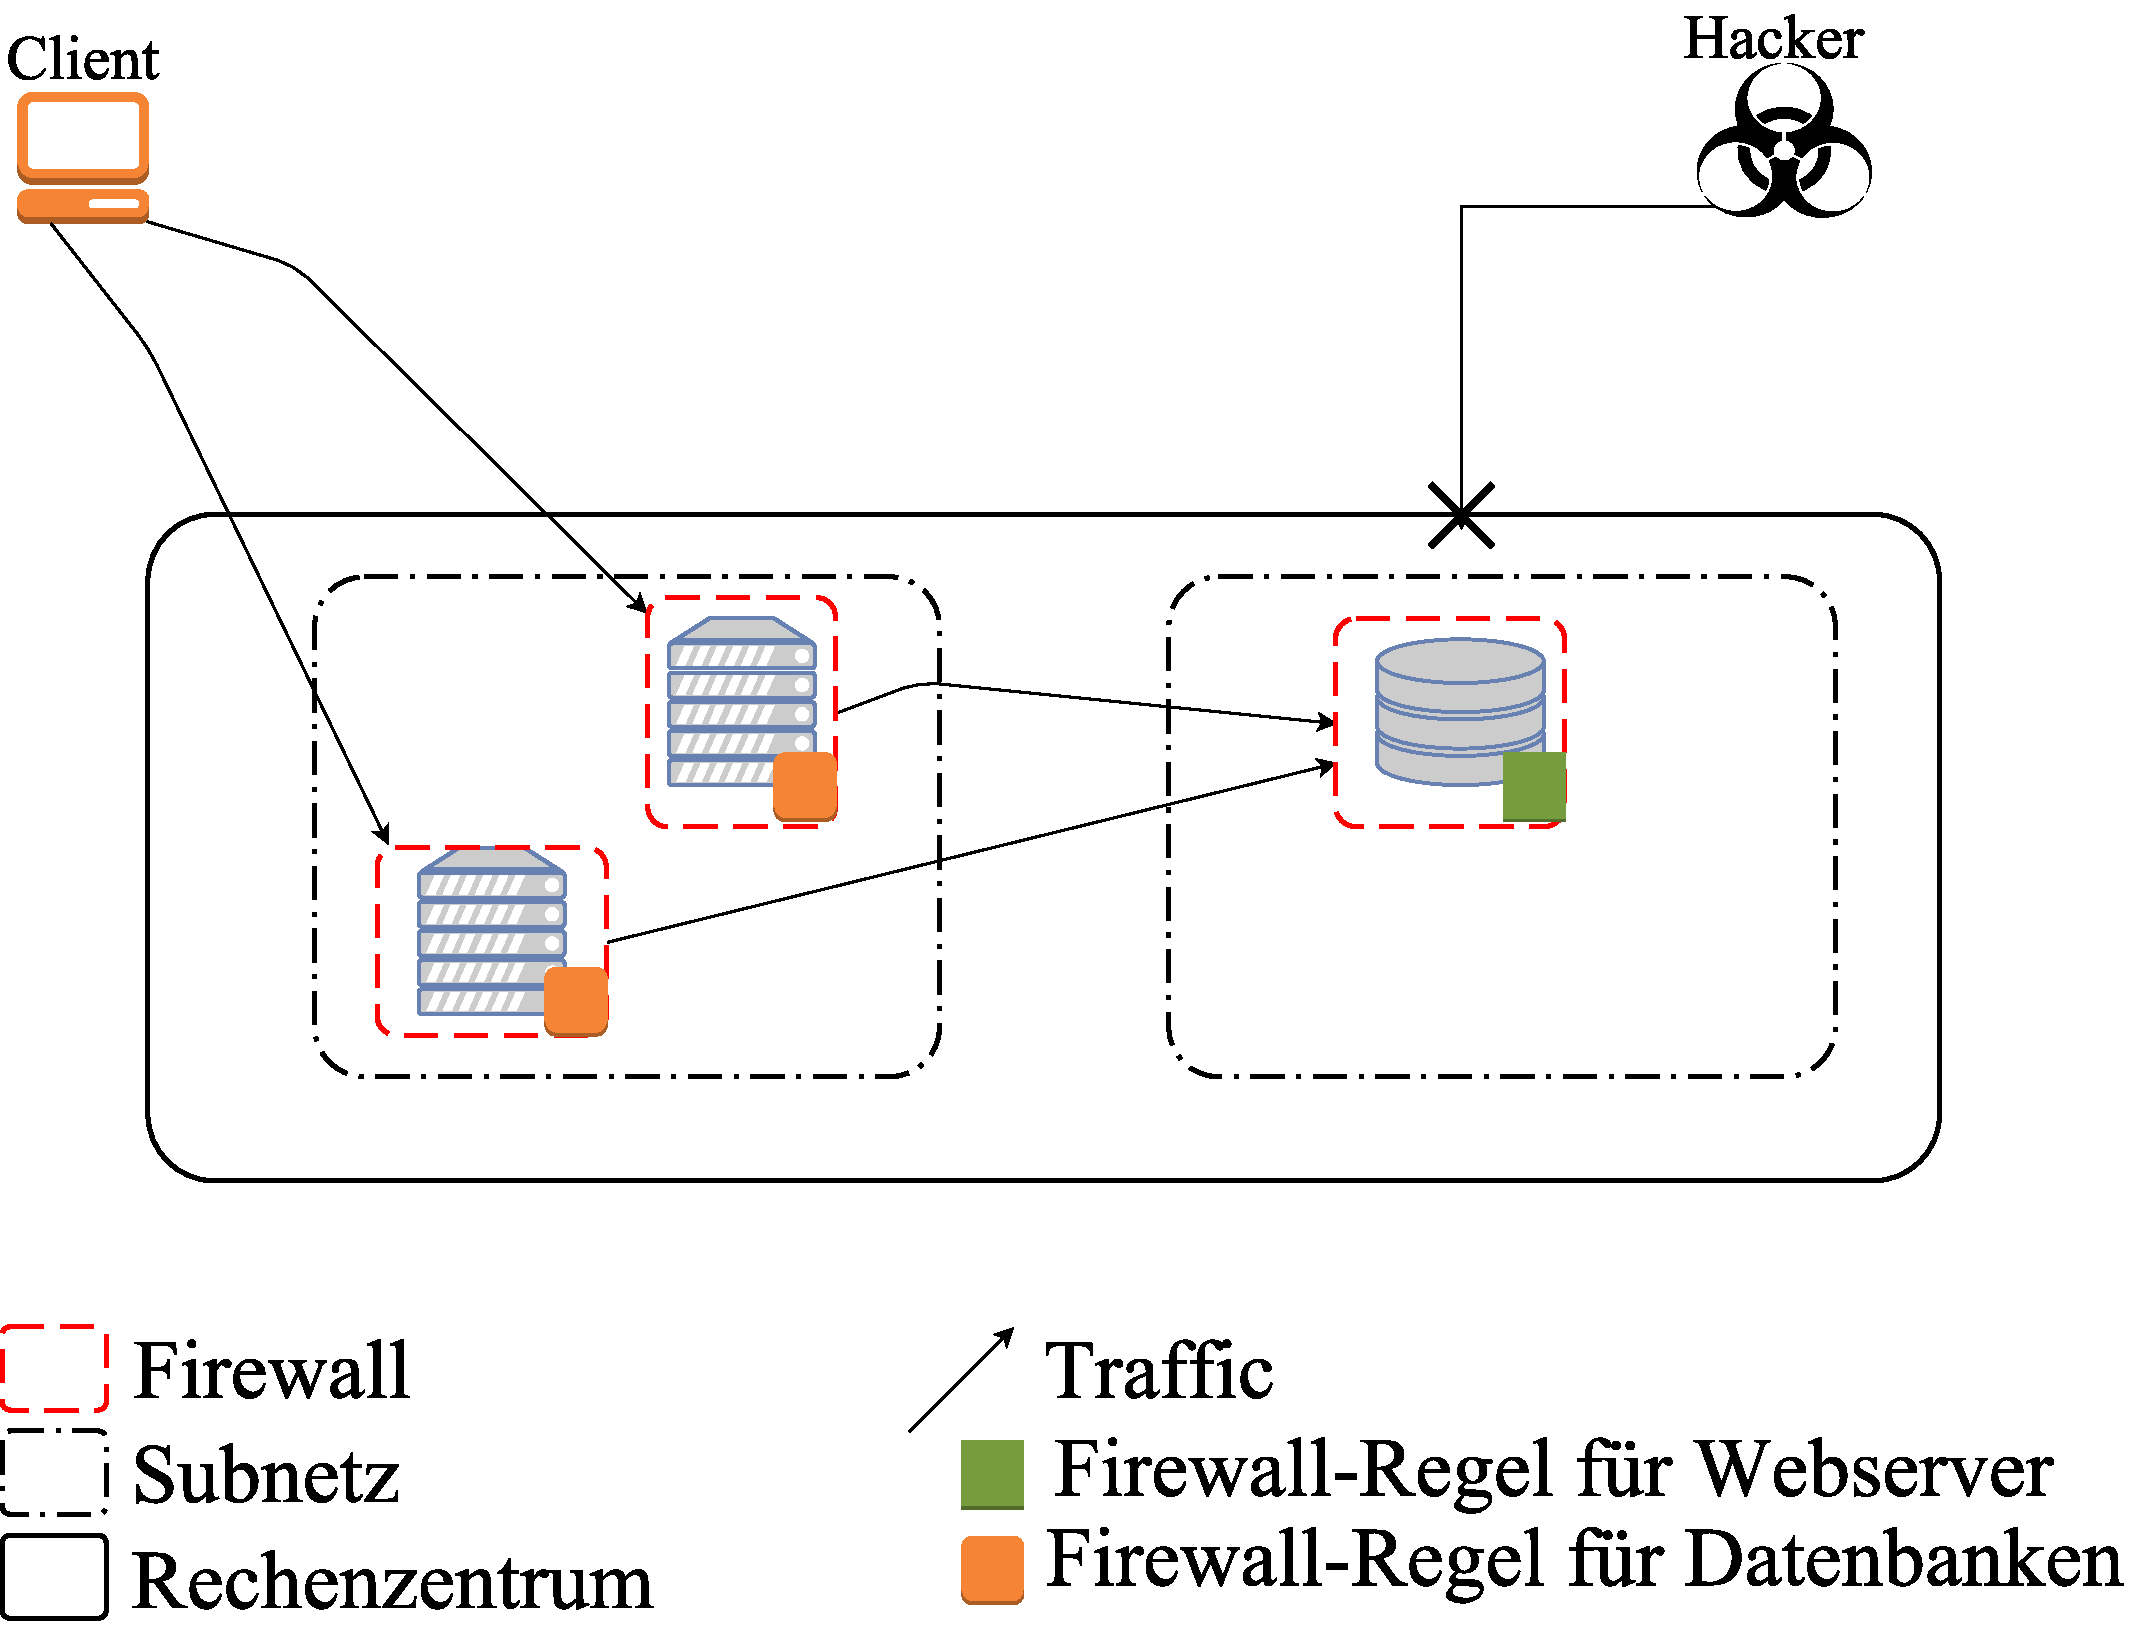
\includegraphics[width=0.8\textwidth]{figures/aws_firewall.pdf}
      \caption{Firewall mit Amazon Security Groups}\label{fig:7}
\end{figure}
\chapter*{Fazit}
Amazon Web Services vereint eine große Palette von Produkten mit einer
weltweiten Infrastruktur. Dadurch lassen sich Applikationen ohne
Probleme weltweit redundant verteilen um eine beinahe perfekte Abdeckung
zu erhalten. Moderne Sicherheitstechnologien wie
Multi\hyp{}Faktor\hyp{}Authentifizierung, Amazon Security Groups und das
Amazon Identiy and Access Management bieten Sicherheit auf hohem Niveau.
Durch die breite Auswahl von Instanzen und Technologien deckt Amazon Web
Services eine breite Kundschaft ab. So sind die einfachen kleineren
Instanzen für Privatkunden interessant, während die mittleren Instanzen
eher für Kleine\hyp{} und Mittelständische Unternehmen gedacht sind. Die
größeren Instanzen eignen sich gut für sehr komplexe Applikationen die
viele Ressourcen benötigen. Die Einteilung in verschiedene Regionen auf
der Welt erweitert nicht nur Amazons Markt sondern unterstützt auch die
Unternehmen, welche sich auf Amazon Web Services verlassen, in ihrem
Bestreben nach immer kleineren Latenzen zum Kunden und damit einer
höheren Kundenzufriedenheit. Außerdem wird durch die zusätzlichen
Regionen eine Ausfallsicherheit hergestellt. Selbst wenn in einem
Rechenzentrum ein Feuer ausbrechen würde wären in der Region eine
handvoll weitere Rechenzentren die den Schaden beim Kunden ausgleichen
würden. Dies wird ermöglicht durch den Kern von Amazon Web Services
Produktpalette: Amazon EC2. Dadurch, dass es sich bei den Instanzen um
Container oder virtuelle Server handelt lassen sich diese relativ
einfach zwischen verschiedenen Rechenzentren oder Regionen verschieben.
Hinzukommend bezahlt der Kunde nur für wirklich eingesetzte Rechenzeit.
Dadurch lassen sich Kosten erheblich senken und es wird ein
Alleinstellungsmerkmal gegenüber andere Cloud\hyp{}Hoster geschaffen,
welche nahezu alle auf monatliche Abonnements von virtuellen Servern und
Containern setzen. Letzteres macht teilweise mehr Sinn für
beispielsweise feste Firmenauftritte in Form von Webseiten. Desweiteren
sind die Kosten auf diese Weise transparenter. Man hat feste Kosten mit
denen man jeden Monat rechnen kann. Wo es bei anderen Hostern allerdings
mangelt ist eine reiche Auswahl an Regionen. Viele Hoster wie
beispielsweise der französische Hoster OVH bieten nur in einer Handvoll Ländern Rechenzentren an
und meistens ist dies dann auch nur das einzige Rechenzentrum in dem
Land. Gerade für Startups können monatliche Abonnements übrigens fatal
sein. Startups haben zu kämpfen mit starken Fluktationen ihrer
Nutzerbasis. So können besonders bei Smartphone Apps mit einem Server
Backend über Nacht mehrere Tausende Nutzer hinzukommen (aber auch
genauso schnell wieder verschwinden). Bei so einem Geschäft auf
monatliche Abonnements zu setzen wäre fatal. Wenn die Nutzerzahlen
nämlich einbrechen wäre man mit hohen Kosten konfrontiert. Deshalb
eignen sich gerade für solche Geschäftsmodelle Amazon EC2 Instanzen.
Durch Amazon EC2 Instanzen kann das jeweilige Startup innerhalb von
Minuten neue Instanzen booten und mit Amazon EC2 Loadbalancern den
Traffic auf die unterschiedlichen Instanzen verteilen. Dies weltweit und
rund um die Uhr. Die Amazon EC2 Weboberfläche gestaltet außerdem die
Administration der Instanzen äußerst einfach. Statt mehreren
Cloud\hyp{}Ingenieuren die einen Openstack\hyp{}Cluster in der eigenen
Firma auf echter Hardware betreuen braucht es bei Amazon EC2 nur einen
Bruchteil der Arbeitskräfte. Dadurch werden nicht nur Personalkosten
gespart (die meistens die größten Kosten im Unternehmen darstellen)
sondern es wird auch die Anschaffung eigener Hardware erspart. Hardware
ist nämlich weit aus schwieriger skalierbar als virtuelle Instanzen.
Wenn sich Firmen dazu entschließen Hardware anzuschaffen ist dies
gekoppelt weiteren Anschaffungen. Man benötigt ein stabiles Stromnetz,
Unterbrechungsfreie Stromversorgungen, einen vernünftigen
Breitbandanschluss, die passenden Räumlichkeiten mit ausreichender
Klimatisierung und Brandschutzbestimmungen. Es kommt also einiges an
Ausgaben zusammen. Eine Alternative wäre die Hardware bei einem
regionalen Anbieter zu mieten. Meistens sind diese regionalen Anbieter
jedoch von der Größe her nicht in der Lage größere Firmen zu betreuen
und es gestaltet sich als schwierig auf schnelle Veränderungen in der
Nutzerbasis zu reagieren. Durch starre Miet\hyp{} und Supportverträge
wird dieser Faktor noch verstärkt.
\addcontentsline{toc}{chapter}{Fazit}
\nocite{*}
\printbibliography
\listoffigures
\end{document}
